\subsection{Tiling Problems}

\begin{eg}
Suppose you are given a 2-by-$n$ area
\begin{center}
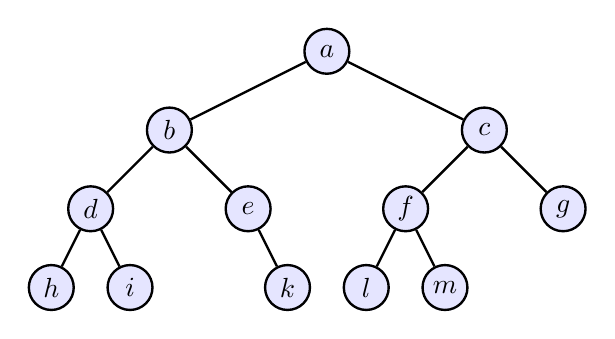
\begin{tikzpicture}

\fill[blue!10] (0.0, 0.0) circle (0.3);
\node [line width=0.03cm,black,minimum size=0.57cm,draw,circle] at (0.0,0.0)(a){};\draw (0.0, 0.0) node[color=black] {$a$};
\fill[blue!10] (-2.0, -1.0) circle (0.3);
\node [line width=0.03cm,black,minimum size=0.57cm,draw,circle] at (-2.0,-1.0)(b){};\draw (-2.0, -1.0) node[color=black] {$b$};
\fill[blue!10] (2.0, -1.0) circle (0.3);
\node [line width=0.03cm,black,minimum size=0.57cm,draw,circle] at (2.0,-1.0)(c){};\draw (2.0, -1.0) node[color=black] {$c$};
\fill[blue!10] (-3.0, -2.0) circle (0.3);
\node [line width=0.03cm,black,minimum size=0.57cm,draw,circle] at (-3.0,-2.0)(d){};\draw (-3.0, -2.0) node[color=black] {$d$};
\fill[blue!10] (-1.0, -2.0) circle (0.3);
\node [line width=0.03cm,black,minimum size=0.57cm,draw,circle] at (-1.0,-2.0)(e){};\draw (-1.0, -2.0) node[color=black] {$e$};
\fill[blue!10] (1.0, -2.0) circle (0.3);
\node [line width=0.03cm,black,minimum size=0.57cm,draw,circle] at (1.0,-2.0)(f){};\draw (1.0, -2.0) node[color=black] {$f$};
\fill[blue!10] (3.0, -2.0) circle (0.3);
\node [line width=0.03cm,black,minimum size=0.57cm,draw,circle] at (3.0,-2.0)(g){};\draw (3.0, -2.0) node[color=black] {$g$};
\fill[blue!10] (-3.5, -3.0) circle (0.3);
\node [line width=0.03cm,black,minimum size=0.57cm,draw,circle] at (-3.5,-3.0)(h){};\draw (-3.5, -3.0) node[color=black] {$h$};
\fill[blue!10] (-2.5, -3.0) circle (0.3);
\node [line width=0.03cm,black,minimum size=0.57cm,draw,circle] at (-2.5,-3.0)(i){};\draw (-2.5, -3.0) node[color=black] {$i$};
\fill[blue!10] (-0.5, -3.0) circle (0.3);
\node [line width=0.03cm,black,minimum size=0.57cm,draw,circle] at (-0.5,-3.0)(k){};\draw (-0.5, -3.0) node[color=black] {$k$};
\fill[blue!10] (0.5, -3.0) circle (0.3);
\node [line width=0.03cm,black,minimum size=0.57cm,draw,circle] at (0.5,-3.0)(l){};\draw (0.5, -3.0) node[color=black] {$l$};
\fill[blue!10] (1.5, -3.0) circle (0.3);
\node [line width=0.03cm,black,minimum size=0.57cm,draw,circle] at (1.5,-3.0)(m){};\draw (1.5, -3.0) node[color=black] {$m$};\draw[line width=0.03cm,black] (a) to  (b);
\draw[line width=0.03cm,black] (a) to  (c);
\draw[line width=0.03cm,black] (b) to  (d);
\draw[line width=0.03cm,black] (b) to  (e);
\draw[line width=0.03cm,black] (c) to  (f);
\draw[line width=0.03cm,black] (c) to  (g);
\draw[line width=0.03cm,black] (d) to  (h);
\draw[line width=0.03cm,black] (d) to  (i);
\draw[line width=0.03cm,black] (e) to  (k);
\draw[line width=0.03cm,black] (f) to  (l);
\draw[line width=0.03cm,black] (f) to  (m);
\end{tikzpicture}

\end{center}


and you need to tile it with 2-by-1 tiles that look like this:
\begin{console}[frame=single, , commandchars=~!@]
...

void insert_head(SLNode ** phead, int i)
{
    *phead = new SLNode(i, *phead);
}

void insert_head(SLNode *& phead, int i)
{
    phead = new SLNode(i, phead);
}

int main()
{
    SLNode * phead = NULL;
    insert_head(&phead, 5);
    print(phead);
    
    return 0;
}
\end{console}

The output is this:
\begin{console}[frame=single,fontsize=\small]
[student@localhost linkedlist] g++ tmp12345678.cpp; ./a.out
<SLNode 0xc01eb0 key:5, next:0>
\end{console}


For instance here's a tiling of a 2-by-5 area:
I put a vertical tile:

\begin{center}
\begin{tikzpicture}[>=triangle 60,shorten >=0.5pt,node distance=2cm,auto,initial text=, double distance=2pt]
\node[state,initial,accepting] (A) at (  0,  0) {$q_0$};

\path[->]
(A) edge [loop above] node {$(a\rightarrow a, S), (b\rightarrow a, S),(\SPACE\rightarrow \SPACE, S), $} ()

;
\end{tikzpicture}
\end{center}
    

And a horizontal tile:
\begin{center}
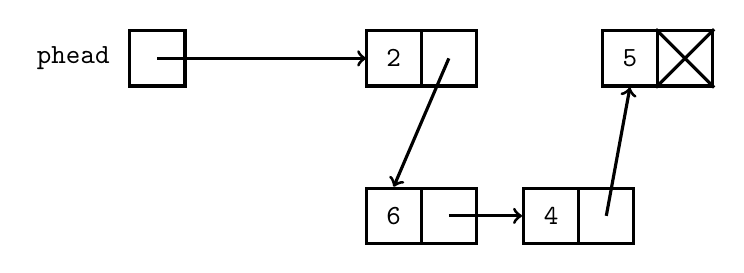
\begin{tikzpicture}

\draw (0.35, 0.35)
  node[draw, line width=0.04cm, , color=black,
       rounded corners=0cm, inner sep=0cm] {

\begin{minipage}[t][0.7cm]{0.7cm}
\mbox{}

\end{minipage}

};\draw (0.35, 0.35) node[color=black] {{\texttt{2}}};
\draw (1.0499999999999998, 0.35)
  node[draw, line width=0.04cm, , color=black,
       rounded corners=0cm, inner sep=0cm] {

\begin{minipage}[t][0.7cm]{0.7cm}
\mbox{}

\end{minipage}

};\draw (1.0499999999999998, 0.35) node[color=black] {{\texttt{}}};
\draw (0.35, -1.65)
  node[draw, line width=0.04cm, , color=black,
       rounded corners=0cm, inner sep=0cm] {

\begin{minipage}[t][0.7cm]{0.7cm}
\mbox{}

\end{minipage}

};\draw (0.35, -1.65) node[color=black] {{\texttt{6}}};
\draw (1.0499999999999998, -1.65)
  node[draw, line width=0.04cm, , color=black,
       rounded corners=0cm, inner sep=0cm] {

\begin{minipage}[t][0.7cm]{0.7cm}
\mbox{}

\end{minipage}

};\draw (1.0499999999999998, -1.65) node[color=black] {{\texttt{}}};
\draw (2.35, -1.65)
  node[draw, line width=0.04cm, , color=black,
       rounded corners=0cm, inner sep=0cm] {

\begin{minipage}[t][0.7cm]{0.7cm}
\mbox{}

\end{minipage}

};\draw (2.35, -1.65) node[color=black] {{\texttt{4}}};
\draw (3.0500000000000003, -1.65)
  node[draw, line width=0.04cm, , color=black,
       rounded corners=0cm, inner sep=0cm] {

\begin{minipage}[t][0.7cm]{0.7cm}
\mbox{}

\end{minipage}

};\draw (3.0500000000000003, -1.65) node[color=black] {{\texttt{}}};
\draw (3.35, 0.35)
  node[draw, line width=0.04cm, , color=black,
       rounded corners=0cm, inner sep=0cm] {

\begin{minipage}[t][0.7cm]{0.7cm}
\mbox{}

\end{minipage}

};\draw (3.35, 0.35) node[color=black] {{\texttt{5}}};
\draw (4.05, 0.35)
  node[draw, line width=0.04cm, , color=black,
       rounded corners=0cm, inner sep=0cm] {

\begin{minipage}[t][0.7cm]{0.7cm}
\mbox{}

\end{minipage}

};\draw (4.05, 0.35) node[color=black] {{\texttt{}}};\draw[line width=0.04cm,black,->] (1.05,0.35) to  (0.35,-1.28);
\draw[line width=0.04cm,black,->] (1.05,-1.65) to  (1.98,-1.65);
\draw[line width=0.04cm,black,->] (3.05,-1.65) to  (3.35,-0.02);
\draw[line width=0.04cm,black] (3.68,0.72) to  (4.42,-0.02);
\draw[line width=0.04cm,black] (4.42,0.72) to  (3.68,-0.02);

\draw (-2.65, 0.35)
  node[draw, line width=0.04cm, , color=black,
       rounded corners=0cm, inner sep=0cm] {

\begin{minipage}[t][0.7cm]{0.7cm}
\mbox{}

\end{minipage}

};\draw (-2.65, 0.35) node[color=black] {{\texttt{}}};\draw[line width=0.04cm,black,->] (-2.65,0.35) to  (0,0.35);

\draw (-3.7199999999999998, 0.35)
  node[draw, line width=0.04cm, , color=white,
       rounded corners=0cm, inner sep=0cm] {

\begin{minipage}[t][0.1cm]{0.1cm}
\mbox{}

\end{minipage}

};\draw (-3.7199999999999998, 0.35) node[color=black] {{\texttt{phead}}};
\end{tikzpicture}

\end{center}


And another horizontal tile:
\begin{center}
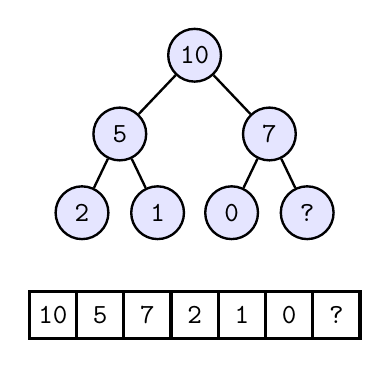
\begin{tikzpicture}

\fill[blue!10] (0.0, 0.0) circle (0.35);
\node [line width=0.03cm,black,minimum size=0.6699999999999999cm,draw,circle] at (0.0,0.0)(10){};\draw (0.0, 0.0) node[color=black] {\texttt{10}};
\fill[blue!10] (-0.95, -1.0) circle (0.35);
\node [line width=0.03cm,black,minimum size=0.6699999999999999cm,draw,circle] at (-0.95,-1.0)(5){};\draw (-0.95, -1.0) node[color=black] {\texttt{5}};
\fill[blue!10] (0.95, -1.0) circle (0.35);
\node [line width=0.03cm,black,minimum size=0.6699999999999999cm,draw,circle] at (0.95,-1.0)(7){};\draw (0.95, -1.0) node[color=black] {\texttt{7}};
\fill[blue!10] (-1.43, -2.0) circle (0.35);
\node [line width=0.03cm,black,minimum size=0.6699999999999999cm,draw,circle] at (-1.43,-2.0)(2){};\draw (-1.43, -2.0) node[color=black] {\texttt{2}};
\fill[blue!10] (-0.47, -2.0) circle (0.35);
\node [line width=0.03cm,black,minimum size=0.6699999999999999cm,draw,circle] at (-0.47,-2.0)(1){};\draw (-0.47, -2.0) node[color=black] {\texttt{1}};
\fill[blue!10] (0.47, -2.0) circle (0.35);
\node [line width=0.03cm,black,minimum size=0.6699999999999999cm,draw,circle] at (0.47,-2.0)(0){};\draw (0.47, -2.0) node[color=black] {\texttt{0}};
\fill[blue!10] (1.43, -2.0) circle (0.35);
\node [line width=0.03cm,black,minimum size=0.6699999999999999cm,draw,circle] at (1.43,-2.0)(?){};\draw (1.43, -2.0) node[color=black] {\texttt{?}};\draw[line width=0.03cm,black] (10) to  (5);
\draw[line width=0.03cm,black] (10) to  (7);
\draw[line width=0.03cm,black] (5) to  (2);
\draw[line width=0.03cm,black] (5) to  (1);
\draw[line width=0.03cm,black] (7) to  (0);
\draw[line width=0.03cm,black] (7) to  (?);

\draw (-1.8, -3.3)
  node[draw, line width=0.04cm, , color=black,
       rounded corners=0cm, inner sep=0cm] {

\begin{minipage}[t][0.6cm]{0.6cm}
\mbox{}

\end{minipage}

};\draw (-1.8, -3.3) node[color=black] {{\texttt{10}}};
\draw (-1.2, -3.3)
  node[draw, line width=0.04cm, , color=black,
       rounded corners=0cm, inner sep=0cm] {

\begin{minipage}[t][0.6cm]{0.6cm}
\mbox{}

\end{minipage}

};\draw (-1.2, -3.3) node[color=black] {{\texttt{5}}};
\draw (-0.6000000000000001, -3.3)
  node[draw, line width=0.04cm, , color=black,
       rounded corners=0cm, inner sep=0cm] {

\begin{minipage}[t][0.6cm]{0.6cm}
\mbox{}

\end{minipage}

};\draw (-0.6000000000000001, -3.3) node[color=black] {{\texttt{7}}};
\draw (-1.1102230246251565e-16, -3.3)
  node[draw, line width=0.04cm, , color=black,
       rounded corners=0cm, inner sep=0cm] {

\begin{minipage}[t][0.6cm]{0.6cm}
\mbox{}

\end{minipage}

};\draw (-1.1102230246251565e-16, -3.3) node[color=black] {{\texttt{2}}};
\draw (0.6, -3.3)
  node[draw, line width=0.04cm, , color=black,
       rounded corners=0cm, inner sep=0cm] {

\begin{minipage}[t][0.6cm]{0.6cm}
\mbox{}

\end{minipage}

};\draw (0.6, -3.3) node[color=black] {{\texttt{1}}};
\draw (1.2, -3.3)
  node[draw, line width=0.04cm, , color=black,
       rounded corners=0cm, inner sep=0cm] {

\begin{minipage}[t][0.6cm]{0.6cm}
\mbox{}

\end{minipage}

};\draw (1.2, -3.3) node[color=black] {{\texttt{0}}};
\draw (1.8, -3.3)
  node[draw, line width=0.04cm, , color=black,
       rounded corners=0cm, inner sep=0cm] {

\begin{minipage}[t][0.6cm]{0.6cm}
\mbox{}

\end{minipage}

};\draw (1.8, -3.3) node[color=black] {{\texttt{?}}};
\end{tikzpicture}

\end{center}


And two vertical tiles:
%-*-latex-*-

\begin{center}
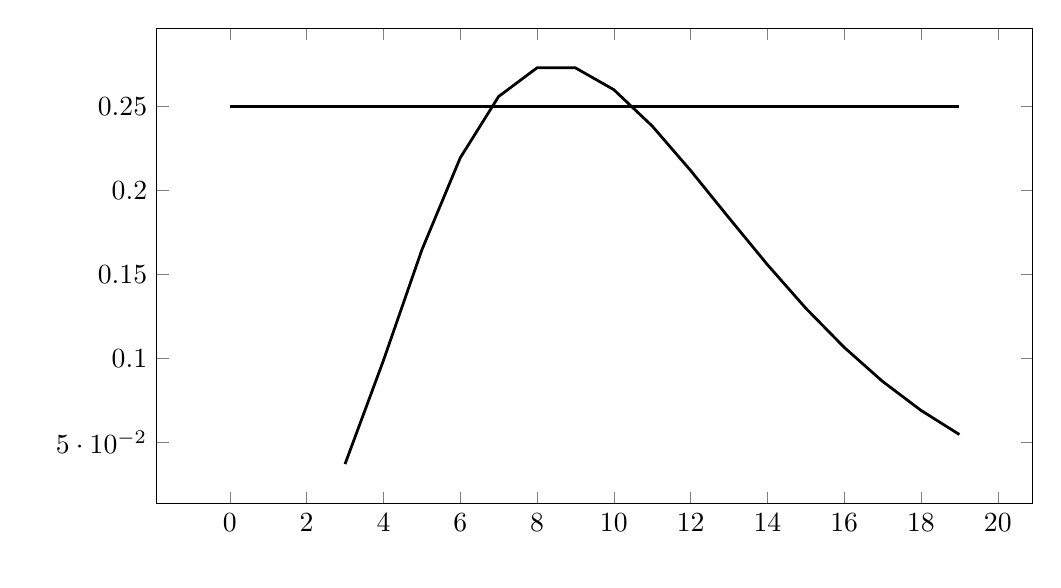
\begin{tikzpicture}[line width=1]
\begin{axis}[width=5in, height=3in,
             scatter/classes={a={mark=*,draw=black}},
             xlabel={\mbox{}},
             xlabel style={name=xlabel}, 
             ylabel={\mbox{}}, 
             legend style={
                at={(xlabel.south)},
                yshift=-1ex,
                anchor=north,
                legend cell align=left,
                },
        ]
]
\addplot[draw=black, line width=1] coordinates {(3, 0.03703703703703703)
(4, 0.0987654320987654)
(5, 0.16460905349794233)
(6, 0.21947873799725642)
(7, 0.2560585276634658)
(8, 0.2731290961743635)
(9, 0.2731290961743635)
(10, 0.26012294873748903)
(11, 0.23844603634269826)
(12, 0.2119520323046207)
(13, 0.18369176133067125)
(14, 0.15585967628056951)
(15, 0.12988306356714127)
(16, 0.10657071882432105)
(17, 0.08627153428635512)
(18, 0.06901722742908409)
(19, 0.05463863838135823)};\addplot[draw=black, line width=1] coordinates {(0, 0.25)
(1, 0.25)
(2, 0.25)
(3, 0.25)
(4, 0.25)
(5, 0.25)
(6, 0.25)
(7, 0.25)
(8, 0.25)
(9, 0.25)
(10, 0.25)
(11, 0.25)
(12, 0.25)
(13, 0.25)
(14, 0.25)
(15, 0.25)
(16, 0.25)
(17, 0.25)
(18, 0.25)
(19, 0.25)};
\end{axis}\end{tikzpicture}\end{center}

There. That's one tiling. Here's another:
\begin{center}
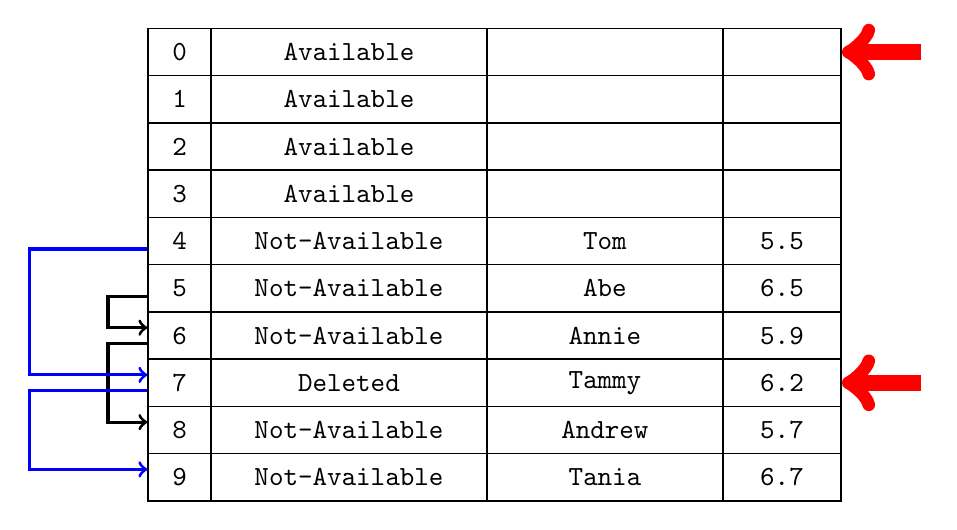
\begin{tikzpicture}

\draw (1.4, 0.7)
  node[draw, line width=0.02cm, , color=black,
       rounded corners=0cm, inner sep=0cm] {

\begin{minipage}[t][0.6cm]{0.8cm}
\mbox{}

\end{minipage}

};\draw (1.4, 0.7) node[color=black] {{\texttt{0}}};
\draw (3.55, 0.7)
  node[draw, line width=0.02cm, , color=black,
       rounded corners=0cm, inner sep=0cm] {

\begin{minipage}[t][0.6cm]{3.5cm}
\mbox{}

\end{minipage}

};\draw (3.55, 0.7) node[color=black] {{\texttt{Available}}};
\draw (6.800000000000001, 0.7)
  node[draw, line width=0.02cm, , color=black,
       rounded corners=0cm, inner sep=0cm] {

\begin{minipage}[t][0.6cm]{3.0cm}
\mbox{}

\end{minipage}

};\draw (6.800000000000001, 0.7) node[color=black] {{\texttt{}}};
\draw (9.05, 0.7)
  node[draw, line width=0.02cm, , color=black,
       rounded corners=0cm, inner sep=0cm] {

\begin{minipage}[t][0.6cm]{1.5cm}
\mbox{}

\end{minipage}

};\draw (9.05, 0.7) node[color=black] {{\texttt{}}};
\draw (1.4, 0.09999999999999987)
  node[draw, line width=0.02cm, , color=black,
       rounded corners=0cm, inner sep=0cm] {

\begin{minipage}[t][0.6cm]{0.8cm}
\mbox{}

\end{minipage}

};\draw (1.4, 0.09999999999999987) node[color=black] {{\texttt{1}}};
\draw (3.55, 0.09999999999999987)
  node[draw, line width=0.02cm, , color=black,
       rounded corners=0cm, inner sep=0cm] {

\begin{minipage}[t][0.6cm]{3.5cm}
\mbox{}

\end{minipage}

};\draw (3.55, 0.09999999999999987) node[color=black] {{\texttt{Available}}};
\draw (6.800000000000001, 0.09999999999999987)
  node[draw, line width=0.02cm, , color=black,
       rounded corners=0cm, inner sep=0cm] {

\begin{minipage}[t][0.6cm]{3.0cm}
\mbox{}

\end{minipage}

};\draw (6.800000000000001, 0.09999999999999987) node[color=black] {{\texttt{}}};
\draw (9.05, 0.09999999999999987)
  node[draw, line width=0.02cm, , color=black,
       rounded corners=0cm, inner sep=0cm] {

\begin{minipage}[t][0.6cm]{1.5cm}
\mbox{}

\end{minipage}

};\draw (9.05, 0.09999999999999987) node[color=black] {{\texttt{}}};
\draw (1.4, -0.5000000000000002)
  node[draw, line width=0.02cm, , color=black,
       rounded corners=0cm, inner sep=0cm] {

\begin{minipage}[t][0.6cm]{0.8cm}
\mbox{}

\end{minipage}

};\draw (1.4, -0.5000000000000002) node[color=black] {{\texttt{2}}};
\draw (3.55, -0.5000000000000002)
  node[draw, line width=0.02cm, , color=black,
       rounded corners=0cm, inner sep=0cm] {

\begin{minipage}[t][0.6cm]{3.5cm}
\mbox{}

\end{minipage}

};\draw (3.55, -0.5000000000000002) node[color=black] {{\texttt{Available}}};
\draw (6.800000000000001, -0.5000000000000002)
  node[draw, line width=0.02cm, , color=black,
       rounded corners=0cm, inner sep=0cm] {

\begin{minipage}[t][0.6cm]{3.0cm}
\mbox{}

\end{minipage}

};\draw (6.800000000000001, -0.5000000000000002) node[color=black] {{\texttt{}}};
\draw (9.05, -0.5000000000000002)
  node[draw, line width=0.02cm, , color=black,
       rounded corners=0cm, inner sep=0cm] {

\begin{minipage}[t][0.6cm]{1.5cm}
\mbox{}

\end{minipage}

};\draw (9.05, -0.5000000000000002) node[color=black] {{\texttt{}}};
\draw (1.4, -1.1000000000000003)
  node[draw, line width=0.02cm, , color=black,
       rounded corners=0cm, inner sep=0cm] {

\begin{minipage}[t][0.6cm]{0.8cm}
\mbox{}

\end{minipage}

};\draw (1.4, -1.1000000000000003) node[color=black] {{\texttt{3}}};
\draw (3.55, -1.1000000000000003)
  node[draw, line width=0.02cm, , color=black,
       rounded corners=0cm, inner sep=0cm] {

\begin{minipage}[t][0.6cm]{3.5cm}
\mbox{}

\end{minipage}

};\draw (3.55, -1.1000000000000003) node[color=black] {{\texttt{Available}}};
\draw (6.800000000000001, -1.1000000000000003)
  node[draw, line width=0.02cm, , color=black,
       rounded corners=0cm, inner sep=0cm] {

\begin{minipage}[t][0.6cm]{3.0cm}
\mbox{}

\end{minipage}

};\draw (6.800000000000001, -1.1000000000000003) node[color=black] {{\texttt{}}};
\draw (9.05, -1.1000000000000003)
  node[draw, line width=0.02cm, , color=black,
       rounded corners=0cm, inner sep=0cm] {

\begin{minipage}[t][0.6cm]{1.5cm}
\mbox{}

\end{minipage}

};\draw (9.05, -1.1000000000000003) node[color=black] {{\texttt{}}};
\draw (1.4, -1.7000000000000002)
  node[draw, line width=0.02cm, , color=black,
       rounded corners=0cm, inner sep=0cm] {

\begin{minipage}[t][0.6cm]{0.8cm}
\mbox{}

\end{minipage}

};\draw (1.4, -1.7000000000000002) node[color=black] {{\texttt{4}}};
\draw (3.55, -1.7000000000000002)
  node[draw, line width=0.02cm, , color=black,
       rounded corners=0cm, inner sep=0cm] {

\begin{minipage}[t][0.6cm]{3.5cm}
\mbox{}

\end{minipage}

};\draw (3.55, -1.7000000000000002) node[color=black] {{\texttt{Not-Available}}};
\draw (6.800000000000001, -1.7000000000000002)
  node[draw, line width=0.02cm, , color=black,
       rounded corners=0cm, inner sep=0cm] {

\begin{minipage}[t][0.6cm]{3.0cm}
\mbox{}

\end{minipage}

};\draw (6.800000000000001, -1.7000000000000002) node[color=black] {{\texttt{Tom}}};
\draw (9.05, -1.7000000000000002)
  node[draw, line width=0.02cm, , color=black,
       rounded corners=0cm, inner sep=0cm] {

\begin{minipage}[t][0.6cm]{1.5cm}
\mbox{}

\end{minipage}

};\draw (9.05, -1.7000000000000002) node[color=black] {{\texttt{5.5}}};
\draw (1.4, -2.3000000000000003)
  node[draw, line width=0.02cm, , color=black,
       rounded corners=0cm, inner sep=0cm] {

\begin{minipage}[t][0.6cm]{0.8cm}
\mbox{}

\end{minipage}

};\draw (1.4, -2.3000000000000003) node[color=black] {{\texttt{5}}};
\draw (3.55, -2.3000000000000003)
  node[draw, line width=0.02cm, , color=black,
       rounded corners=0cm, inner sep=0cm] {

\begin{minipage}[t][0.6cm]{3.5cm}
\mbox{}

\end{minipage}

};\draw (3.55, -2.3000000000000003) node[color=black] {{\texttt{Not-Available}}};
\draw (6.800000000000001, -2.3000000000000003)
  node[draw, line width=0.02cm, , color=black,
       rounded corners=0cm, inner sep=0cm] {

\begin{minipage}[t][0.6cm]{3.0cm}
\mbox{}

\end{minipage}

};\draw (6.800000000000001, -2.3000000000000003) node[color=black] {{\texttt{Abe}}};
\draw (9.05, -2.3000000000000003)
  node[draw, line width=0.02cm, , color=black,
       rounded corners=0cm, inner sep=0cm] {

\begin{minipage}[t][0.6cm]{1.5cm}
\mbox{}

\end{minipage}

};\draw (9.05, -2.3000000000000003) node[color=black] {{\texttt{6.5}}};
\draw (1.4, -2.9000000000000004)
  node[draw, line width=0.02cm, , color=black,
       rounded corners=0cm, inner sep=0cm] {

\begin{minipage}[t][0.6cm]{0.8cm}
\mbox{}

\end{minipage}

};\draw (1.4, -2.9000000000000004) node[color=black] {{\texttt{6}}};
\draw (3.55, -2.9000000000000004)
  node[draw, line width=0.02cm, , color=black,
       rounded corners=0cm, inner sep=0cm] {

\begin{minipage}[t][0.6cm]{3.5cm}
\mbox{}

\end{minipage}

};\draw (3.55, -2.9000000000000004) node[color=black] {{\texttt{Not-Available}}};
\draw (6.800000000000001, -2.9000000000000004)
  node[draw, line width=0.02cm, , color=black,
       rounded corners=0cm, inner sep=0cm] {

\begin{minipage}[t][0.6cm]{3.0cm}
\mbox{}

\end{minipage}

};\draw (6.800000000000001, -2.9000000000000004) node[color=black] {{\texttt{Annie}}};
\draw (9.05, -2.9000000000000004)
  node[draw, line width=0.02cm, , color=black,
       rounded corners=0cm, inner sep=0cm] {

\begin{minipage}[t][0.6cm]{1.5cm}
\mbox{}

\end{minipage}

};\draw (9.05, -2.9000000000000004) node[color=black] {{\texttt{5.9}}};
\draw (1.4, -3.500000000000001)
  node[draw, line width=0.02cm, , color=black,
       rounded corners=0cm, inner sep=0cm] {

\begin{minipage}[t][0.6cm]{0.8cm}
\mbox{}

\end{minipage}

};\draw (1.4, -3.500000000000001) node[color=black] {{\texttt{7}}};
\draw (3.55, -3.500000000000001)
  node[draw, line width=0.02cm, , color=black,
       rounded corners=0cm, inner sep=0cm] {

\begin{minipage}[t][0.6cm]{3.5cm}
\mbox{}

\end{minipage}

};\draw (3.55, -3.500000000000001) node[color=black] {{\texttt{Deleted}}};
\draw (6.800000000000001, -3.500000000000001)
  node[draw, line width=0.02cm, , color=black,
       rounded corners=0cm, inner sep=0cm] {

\begin{minipage}[t][0.6cm]{3.0cm}
\mbox{}

\end{minipage}

};\draw (6.800000000000001, -3.500000000000001) node[color=black] {{\texttt{Tammy}}};
\draw (9.05, -3.500000000000001)
  node[draw, line width=0.02cm, , color=black,
       rounded corners=0cm, inner sep=0cm] {

\begin{minipage}[t][0.6cm]{1.5cm}
\mbox{}

\end{minipage}

};\draw (9.05, -3.500000000000001) node[color=black] {{\texttt{6.2}}};
\draw (1.4, -4.1000000000000005)
  node[draw, line width=0.02cm, , color=black,
       rounded corners=0cm, inner sep=0cm] {

\begin{minipage}[t][0.6cm]{0.8cm}
\mbox{}

\end{minipage}

};\draw (1.4, -4.1000000000000005) node[color=black] {{\texttt{8}}};
\draw (3.55, -4.1000000000000005)
  node[draw, line width=0.02cm, , color=black,
       rounded corners=0cm, inner sep=0cm] {

\begin{minipage}[t][0.6cm]{3.5cm}
\mbox{}

\end{minipage}

};\draw (3.55, -4.1000000000000005) node[color=black] {{\texttt{Not-Available}}};
\draw (6.800000000000001, -4.1000000000000005)
  node[draw, line width=0.02cm, , color=black,
       rounded corners=0cm, inner sep=0cm] {

\begin{minipage}[t][0.6cm]{3.0cm}
\mbox{}

\end{minipage}

};\draw (6.800000000000001, -4.1000000000000005) node[color=black] {{\texttt{Andrew}}};
\draw (9.05, -4.1000000000000005)
  node[draw, line width=0.02cm, , color=black,
       rounded corners=0cm, inner sep=0cm] {

\begin{minipage}[t][0.6cm]{1.5cm}
\mbox{}

\end{minipage}

};\draw (9.05, -4.1000000000000005) node[color=black] {{\texttt{5.7}}};
\draw (1.4, -4.7)
  node[draw, line width=0.02cm, , color=black,
       rounded corners=0cm, inner sep=0cm] {

\begin{minipage}[t][0.6cm]{0.8cm}
\mbox{}

\end{minipage}

};\draw (1.4, -4.7) node[color=black] {{\texttt{9}}};
\draw (3.55, -4.7)
  node[draw, line width=0.02cm, , color=black,
       rounded corners=0cm, inner sep=0cm] {

\begin{minipage}[t][0.6cm]{3.5cm}
\mbox{}

\end{minipage}

};\draw (3.55, -4.7) node[color=black] {{\texttt{Not-Available}}};
\draw (6.800000000000001, -4.7)
  node[draw, line width=0.02cm, , color=black,
       rounded corners=0cm, inner sep=0cm] {

\begin{minipage}[t][0.6cm]{3.0cm}
\mbox{}

\end{minipage}

};\draw (6.800000000000001, -4.7) node[color=black] {{\texttt{Tania}}};
\draw (9.05, -4.7)
  node[draw, line width=0.02cm, , color=black,
       rounded corners=0cm, inner sep=0cm] {

\begin{minipage}[t][0.6cm]{1.5cm}
\mbox{}

\end{minipage}

};\draw (9.05, -4.7) node[color=black] {{\texttt{6.7}}};\draw[line width=0.04cm,black,->] (0.99,-2.4) to  (0.49,-2.4) to  (0.49,-2.8) to  (0.99,-2.8);
\draw[line width=0.04cm,black,->] (0.99,-3.0) to  (0.49,-3.0) to  (0.49,-4.0) to  (0.99,-4.0);
\draw[line width=0.04cm,blue,->] (0.99,-1.8) to  (-0.51,-1.8) to  (-0.51,-3.4) to  (0.99,-3.4);
\draw[line width=0.04cm,blue,->] (0.99,-3.6) to  (-0.51,-3.6) to  (-0.51,-4.6) to  (0.99,-4.6);
\draw[line width=0.2cm,red,->] (10.81,-3.5) to  (9.81,-3.5);
\draw[line width=0.2cm,red,->] (10.81,0.7) to  (9.81,0.7);
\end{tikzpicture}

\end{center}


Now let $a_n$ be the number of tilings
for a 2-by-$n$ area.
Compute $a_{20}$
Of course instead of trying to draw all the diagram up to $n = 20$,
you probably want to find a recurrence relation and then use the
recurrence relation to compute $a_{20}$.
It's even better if you can find a closed form for $a_n$ -- but
we'll do that later.
Before first you should do some experiments.
\begin{enumerate}[nosep]
  \item[(a)] Draw all the tilings for $n=1, 2, 3, 4, 5$.
  \item[(b)] Find a recurrence relation for $a_n$.
\end{enumerate}
\end{eg}

\textsc{Solution.}

(a) is simple. I'll leave that to you.

(b)
This problem is recursive, i.e., the problem of
tiling the 2-by-$n$ area contains the same problem(s), but with a
smaller area.
Here's a 2-by-$n$ area:
\begin{center}
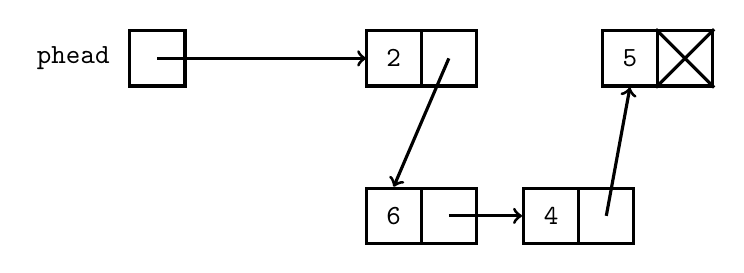
\begin{tikzpicture}

\draw (0.35, 0.35)
  node[draw, line width=0.04cm, , color=black,
       rounded corners=0cm, inner sep=0cm] {

\begin{minipage}[t][0.7cm]{0.7cm}
\mbox{}

\end{minipage}

};\draw (0.35, 0.35) node[color=black] {{\texttt{2}}};
\draw (1.0499999999999998, 0.35)
  node[draw, line width=0.04cm, , color=black,
       rounded corners=0cm, inner sep=0cm] {

\begin{minipage}[t][0.7cm]{0.7cm}
\mbox{}

\end{minipage}

};\draw (1.0499999999999998, 0.35) node[color=black] {{\texttt{}}};
\draw (0.35, -1.65)
  node[draw, line width=0.04cm, , color=black,
       rounded corners=0cm, inner sep=0cm] {

\begin{minipage}[t][0.7cm]{0.7cm}
\mbox{}

\end{minipage}

};\draw (0.35, -1.65) node[color=black] {{\texttt{6}}};
\draw (1.0499999999999998, -1.65)
  node[draw, line width=0.04cm, , color=black,
       rounded corners=0cm, inner sep=0cm] {

\begin{minipage}[t][0.7cm]{0.7cm}
\mbox{}

\end{minipage}

};\draw (1.0499999999999998, -1.65) node[color=black] {{\texttt{}}};
\draw (2.35, -1.65)
  node[draw, line width=0.04cm, , color=black,
       rounded corners=0cm, inner sep=0cm] {

\begin{minipage}[t][0.7cm]{0.7cm}
\mbox{}

\end{minipage}

};\draw (2.35, -1.65) node[color=black] {{\texttt{4}}};
\draw (3.0500000000000003, -1.65)
  node[draw, line width=0.04cm, , color=black,
       rounded corners=0cm, inner sep=0cm] {

\begin{minipage}[t][0.7cm]{0.7cm}
\mbox{}

\end{minipage}

};\draw (3.0500000000000003, -1.65) node[color=black] {{\texttt{}}};
\draw (3.35, 0.35)
  node[draw, line width=0.04cm, , color=black,
       rounded corners=0cm, inner sep=0cm] {

\begin{minipage}[t][0.7cm]{0.7cm}
\mbox{}

\end{minipage}

};\draw (3.35, 0.35) node[color=black] {{\texttt{5}}};
\draw (4.05, 0.35)
  node[draw, line width=0.04cm, , color=black,
       rounded corners=0cm, inner sep=0cm] {

\begin{minipage}[t][0.7cm]{0.7cm}
\mbox{}

\end{minipage}

};\draw (4.05, 0.35) node[color=black] {{\texttt{}}};\draw[line width=0.04cm,black,->] (1.05,0.35) to  (0.35,-1.28);
\draw[line width=0.04cm,black,->] (1.05,-1.65) to  (1.98,-1.65);
\draw[line width=0.04cm,black,->] (3.05,-1.65) to  (3.35,-0.02);
\draw[line width=0.04cm,black] (3.68,0.72) to  (4.42,-0.02);
\draw[line width=0.04cm,black] (4.42,0.72) to  (3.68,-0.02);

\draw (-2.65, 0.35)
  node[draw, line width=0.04cm, , color=black,
       rounded corners=0cm, inner sep=0cm] {

\begin{minipage}[t][0.7cm]{0.7cm}
\mbox{}

\end{minipage}

};\draw (-2.65, 0.35) node[color=black] {{\texttt{}}};\draw[line width=0.04cm,black,->] (-2.65,0.35) to  (0,0.35);

\draw (-3.7199999999999998, 0.35)
  node[draw, line width=0.04cm, , color=white,
       rounded corners=0cm, inner sep=0cm] {

\begin{minipage}[t][0.1cm]{0.1cm}
\mbox{}

\end{minipage}

};\draw (-3.7199999999999998, 0.35) node[color=black] {{\texttt{phead}}};
\end{tikzpicture}

\end{center}



The left side of this area is either tiled by a vertical tile:
\begin{center}
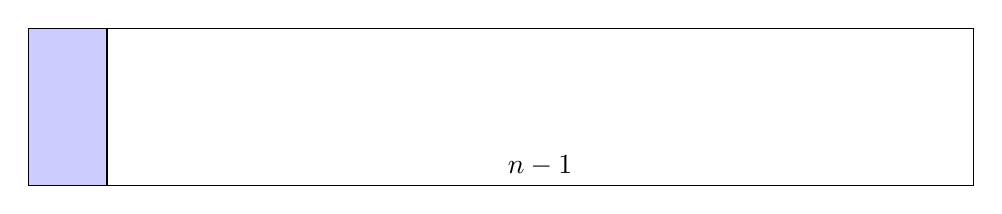
\begin{tikzpicture}

\draw (6.0, 1.0)
  node[draw, , , color=black,
       rounded corners=0cm, inner sep=0cm] {

\begin{minipage}[t][2cm]{12cm}
\mbox{}

\end{minipage}

};
\draw (0.5, 1.0)
  node[fill=blue!20!white,rounded corners=0cm,inner sep=0cm] {

\begin{minipage}[t][2cm]{1cm}
\mbox{}

\end{minipage}

};
\draw (0.5, 1.0)
  node[draw, , , color=black,
       rounded corners=0cm, inner sep=0cm] {

\begin{minipage}[t][2cm]{1cm}
\mbox{}

\end{minipage}

};
\draw (6.5, 0.25)
  node[draw=none, line width=0cm, , color=black,
       rounded corners=0cm, inner sep=0cm] {

\begin{minipage}[t][0.1cm]{0.1cm}
\mbox{}

\end{minipage}

};\draw (6.5, 0.25) node[color=black] {$n - 1$};
\end{tikzpicture}

\end{center}


or by two horizontal tiles:
\begin{center}
\begin{tikzpicture}

\fill[blue!10] (0.0, 0.0) circle (0.3);
\node [line width=0.03cm,black,minimum size=0.57cm,draw,circle] at (0.0,0.0)(a){};\draw (0.0, 0.0) node[color=black] {$a$};
\fill[blue!10] (-2.0, -1.0) circle (0.3);
\node [line width=0.03cm,black,minimum size=0.57cm,draw,circle] at (-2.0,-1.0)(b){};\draw (-2.0, -1.0) node[color=black] {$b$};
\fill[blue!10] (2.0, -1.0) circle (0.3);
\node [line width=0.03cm,black,minimum size=0.57cm,draw,circle] at (2.0,-1.0)(d){};\draw (2.0, -1.0) node[color=black] {$d$};
\fill[blue!10] (-3.0, -2.0) circle (0.3);
\node [line width=0.03cm,black,minimum size=0.57cm,draw,circle] at (-3.0,-2.0)(e){};\draw (-3.0, -2.0) node[color=black] {$e$};
\fill[blue!10] (-1.0, -2.0) circle (0.3);
\node [line width=0.03cm,black,minimum size=0.57cm,draw,circle] at (-1.0,-2.0)(f){};\draw (-1.0, -2.0) node[color=black] {$f$};
\fill[blue!10] (1.0, -2.0) circle (0.3);
\node [line width=0.03cm,black,minimum size=0.57cm,draw,circle] at (1.0,-2.0)(h){};\draw (1.0, -2.0) node[color=black] {$h$};
\fill[blue!10] (3.0, -2.0) circle (0.3);
\node [line width=0.03cm,black,minimum size=0.57cm,draw,circle] at (3.0,-2.0)(o){};\draw (3.0, -2.0) node[color=black] {$o$};
\fill[blue!10] (-2.5, -3.0) circle (0.3);
\node [line width=0.03cm,black,minimum size=0.57cm,draw,circle] at (-2.5,-3.0)(l){};\draw (-2.5, -3.0) node[color=black] {$l$};
\fill[blue!10] (1.5, -3.0) circle (0.3);
\node [line width=0.03cm,black,minimum size=0.57cm,draw,circle] at (1.5,-3.0)(m){};\draw (1.5, -3.0) node[color=black] {$m$};
\fill[blue!10] (3.5, -3.0) circle (0.3);
\node [line width=0.03cm,black,minimum size=0.57cm,draw,circle] at (3.5,-3.0)(j){};\draw (3.5, -3.0) node[color=black] {$j$};\draw[line width=0.03cm,black,->,>=triangle 60] (a) to  (b);
\draw[line width=0.03cm,black,->,>=triangle 60] (a) to  (d);
\draw[line width=0.03cm,black,->,>=triangle 60] (b) to  (e);
\draw[line width=0.03cm,black,->,>=triangle 60] (b) to  (f);
\draw[line width=0.03cm,black,->,>=triangle 60] (d) to  (h);
\draw[line width=0.03cm,black,->,>=triangle 60] (d) to  (o);
\draw[line width=0.03cm,black,->,>=triangle 60] (e) to  (l);
\draw[line width=0.03cm,black,->,>=triangle 60] (h) to  (m);
\draw[line width=0.03cm,black,->,>=triangle 60] (o) to  (j);
\end{tikzpicture}

\end{center}



In the first case, the resulting area to to be tiled is a 2-by-($n-1$) area.
\begin{center}
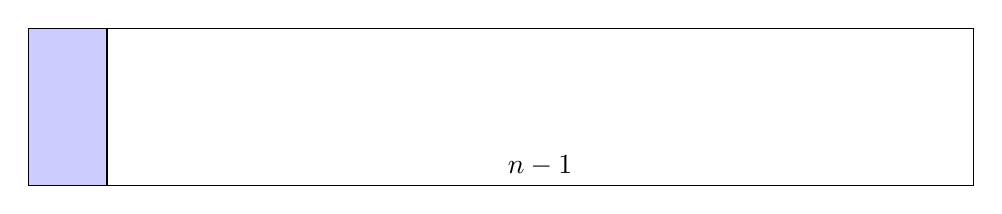
\begin{tikzpicture}

\draw (6.0, 1.0)
  node[draw, , , color=black,
       rounded corners=0cm, inner sep=0cm] {

\begin{minipage}[t][2cm]{12cm}
\mbox{}

\end{minipage}

};
\draw (0.5, 1.0)
  node[fill=blue!20!white,rounded corners=0cm,inner sep=0cm] {

\begin{minipage}[t][2cm]{1cm}
\mbox{}

\end{minipage}

};
\draw (0.5, 1.0)
  node[draw, , , color=black,
       rounded corners=0cm, inner sep=0cm] {

\begin{minipage}[t][2cm]{1cm}
\mbox{}

\end{minipage}

};
\draw (6.5, 0.25)
  node[draw=none, line width=0cm, , color=black,
       rounded corners=0cm, inner sep=0cm] {

\begin{minipage}[t][0.1cm]{0.1cm}
\mbox{}

\end{minipage}

};\draw (6.5, 0.25) node[color=black] {$n - 1$};
\end{tikzpicture}

\end{center}


and clearly the number of ways to tile the remaining untiled area
is the number of ways to tile a 2-by-($n-1$) area.
Hence there are $a_{n-1}$ to tile the 2-by-$n$ area assuming that we
start with a vertical tile.

Likewise, in the second case,
the resulting area to be tiled is a 2-by-($n-2$) area.
\begin{center}
\begin{tikzpicture}

\fill[blue!10] (0.0, 0.0) circle (0.3);
\node [line width=0.03cm,black,minimum size=0.57cm,draw,circle] at (0.0,0.0)(a){};\draw (0.0, 0.0) node[color=black] {$a$};
\fill[blue!10] (-2.0, -1.0) circle (0.3);
\node [line width=0.03cm,black,minimum size=0.57cm,draw,circle] at (-2.0,-1.0)(b){};\draw (-2.0, -1.0) node[color=black] {$b$};
\fill[blue!10] (2.0, -1.0) circle (0.3);
\node [line width=0.03cm,black,minimum size=0.57cm,draw,circle] at (2.0,-1.0)(d){};\draw (2.0, -1.0) node[color=black] {$d$};
\fill[blue!10] (-3.0, -2.0) circle (0.3);
\node [line width=0.03cm,black,minimum size=0.57cm,draw,circle] at (-3.0,-2.0)(e){};\draw (-3.0, -2.0) node[color=black] {$e$};
\fill[blue!10] (-1.0, -2.0) circle (0.3);
\node [line width=0.03cm,black,minimum size=0.57cm,draw,circle] at (-1.0,-2.0)(f){};\draw (-1.0, -2.0) node[color=black] {$f$};
\fill[blue!10] (1.0, -2.0) circle (0.3);
\node [line width=0.03cm,black,minimum size=0.57cm,draw,circle] at (1.0,-2.0)(m){};\draw (1.0, -2.0) node[color=black] {$m$};
\fill[blue!10] (3.0, -2.0) circle (0.3);
\node [line width=0.03cm,black,minimum size=0.57cm,draw,circle] at (3.0,-2.0)(o){};\draw (3.0, -2.0) node[color=black] {$o$};
\fill[blue!10] (-3.5, -3.0) circle (0.3);
\node [line width=0.03cm,black,minimum size=0.57cm,draw,circle] at (-3.5,-3.0)(k){};\draw (-3.5, -3.0) node[color=black] {$k$};
\fill[blue!10] (-2.5, -3.0) circle (0.3);
\node [line width=0.03cm,black,minimum size=0.57cm,draw,circle] at (-2.5,-3.0)(l){};\draw (-2.5, -3.0) node[color=black] {$l$};
\fill[blue!10] (3.5, -3.0) circle (0.3);
\node [line width=0.03cm,black,minimum size=0.57cm,draw,circle] at (3.5,-3.0)(j){};\draw (3.5, -3.0) node[color=black] {$j$};\draw[line width=0.03cm,black,->,>=triangle 60] (a) to  (b);
\draw[line width=0.03cm,black,->,>=triangle 60] (a) to  (d);
\draw[line width=0.03cm,black,->,>=triangle 60] (b) to  (e);
\draw[line width=0.03cm,black,->,>=triangle 60] (b) to  (f);
\draw[line width=0.03cm,black,->,>=triangle 60] (d) to  (m);
\draw[line width=0.03cm,black,->,>=triangle 60] (d) to  (o);
\draw[line width=0.03cm,black,->,>=triangle 60] (e) to  (k);
\draw[line width=0.03cm,black,->,>=triangle 60] (e) to  (l);
\draw[line width=0.03cm,black,->,>=triangle 60] (o) to  (j);
\end{tikzpicture}

\end{center}


and therefore the number of ways to the 2-by-$n$ area assuming that
we start with two horizontal tiles is $a_{n-2}$.

Altogether, since a tiling of the 2-by-$n$ area must be one of the two cases
above and since the above two cases
of tilings do not have any tiling in common, by the addition principle,
the total number of ways to tile the 2-by-$n$ area is
\[
a_n = a_{n-1} + a_{n-2}
\]
for $n \geq 2$.
Note that
\[
a_1 = 1
\]
Also, it's easy to see that
\[
a_2 = 2
\]
Hence from $a_2 = a_1 + a_0$, we get
\[
2 = 1 + a_0
\]
i.e. $a_0 = 1$.
Therefore we have
\[
a_n =
\begin{cases}
1 & \text{ if } n = 0, 1 \\
a_{n-1} + a_{n - 2} &\text{ if } n \geq 2
\end{cases}
\]
\qed

Does it surprise you that the above is the Fibonacci recurrence relation?

%Your job: find a closed form for $a_n$.

%-*-latex-*-

\begin{ex} 
  \label{ex:prob-00}
  \tinysidebar{\debug{exercises/{disc-prob-28/question.tex}}}

  \solutionlink{sol:prob-00}
  \qed
\end{ex} 
\begin{python0}
from solutions import *
add(label="ex:prob-00",
    srcfilename='exercises/discrete-probability/prob-00/answer.tex') 
\end{python0}


\newpage%-*-latex-*-

\begin{ex} 
  \label{ex:prob-00}
  \tinysidebar{\debug{exercises/{disc-prob-28/question.tex}}}

  \solutionlink{sol:prob-00}
  \qed
\end{ex} 
\begin{python0}
from solutions import *
add(label="ex:prob-00",
    srcfilename='exercises/discrete-probability/prob-00/answer.tex') 
\end{python0}

\newpage%-*-latex-*-

\begin{ex} 
  \label{ex:prob-00}
  \tinysidebar{\debug{exercises/{disc-prob-28/question.tex}}}

  \solutionlink{sol:prob-00}
  \qed
\end{ex} 
\begin{python0}
from solutions import *
add(label="ex:prob-00",
    srcfilename='exercises/discrete-probability/prob-00/answer.tex') 
\end{python0}

\newpage%-*-latex-*-

\begin{ex} 
  \label{ex:prob-00}
  \tinysidebar{\debug{exercises/{disc-prob-28/question.tex}}}

  \solutionlink{sol:prob-00}
  \qed
\end{ex} 
\begin{python0}
from solutions import *
add(label="ex:prob-00",
    srcfilename='exercises/discrete-probability/prob-00/answer.tex') 
\end{python0}

\newpage%-*-latex-*-

\begin{ex} 
  \label{ex:prob-00}
  \tinysidebar{\debug{exercises/{disc-prob-28/question.tex}}}

  \solutionlink{sol:prob-00}
  \qed
\end{ex} 
\begin{python0}
from solutions import *
add(label="ex:prob-00",
    srcfilename='exercises/discrete-probability/prob-00/answer.tex') 
\end{python0}

%-*-latex-*-

\begin{ex} 
  \label{ex:prob-00}
  \tinysidebar{\debug{exercises/{disc-prob-28/question.tex}}}

  \solutionlink{sol:prob-00}
  \qed
\end{ex} 
\begin{python0}
from solutions import *
add(label="ex:prob-00",
    srcfilename='exercises/discrete-probability/prob-00/answer.tex') 
\end{python0}

%-*-latex-*-

\begin{ex} 
  \label{ex:prob-00}
  \tinysidebar{\debug{exercises/{disc-prob-28/question.tex}}}

  \solutionlink{sol:prob-00}
  \qed
\end{ex} 
\begin{python0}
from solutions import *
add(label="ex:prob-00",
    srcfilename='exercises/discrete-probability/prob-00/answer.tex') 
\end{python0}

